\section{Diskussion} 
\begin{frame}{Ændringer i billedet}

	\begin{itemize}
		\setlength\itemsep{1em}
		\item Minimere antal ændringer i pixels
		\item For let at se i histogram
		\begin{itemize}
			\vspace*{1em}
			\setlength\itemsep{1em}
			\item<con@1->[$\times$] Ændring i pixelfarve
			\item<pro@1->[\checkmark] Pixelombytninger
		\end{itemize}
	\end{itemize}
\end{frame}

% Grunden til cover og GT er lidt forskellige
% er pga. de få forces, der er.
% Hvis GT udelukkende havde brugt switches,
% havde histogrammerne været ens.
\begin{frame}{Ændringer i billedet}
	\begin{figure}
		\centering
		\begin{center}
		\subfigure[JPEG u. besked]{\label{fig:a}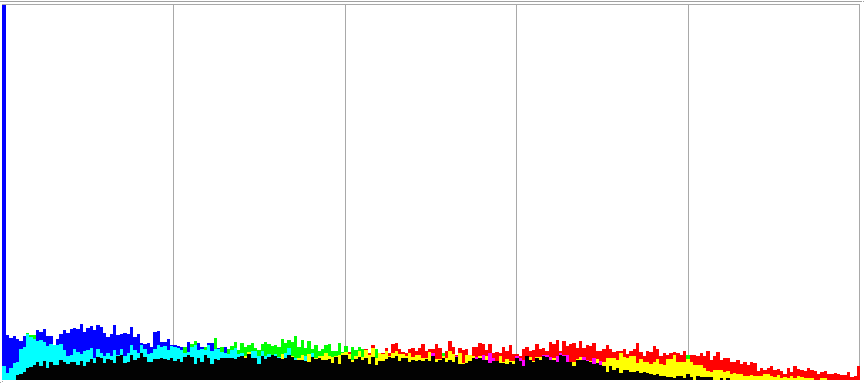
\includegraphics[width=.4\textwidth]{figures/gtOut2Histo.png}}
		\end{center}
		~
		\subfigure[LSB m. besked]{\label{fig:b}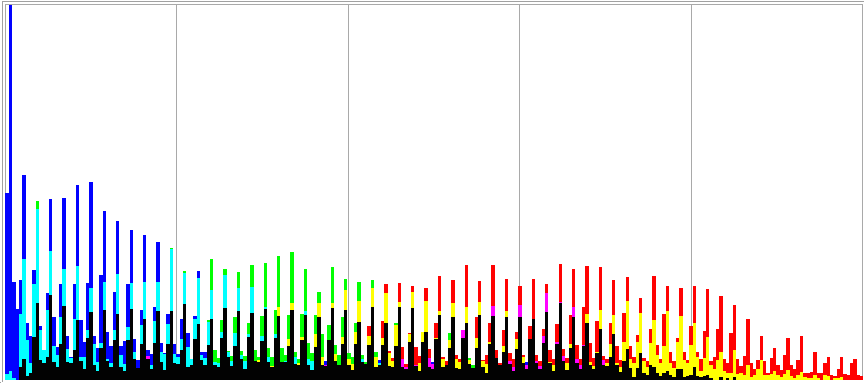
\includegraphics[width=.4\textwidth]{figures/lsbOutHisto.png}}
		~
		\subfigure[GT m. besked]{\label{fig:c}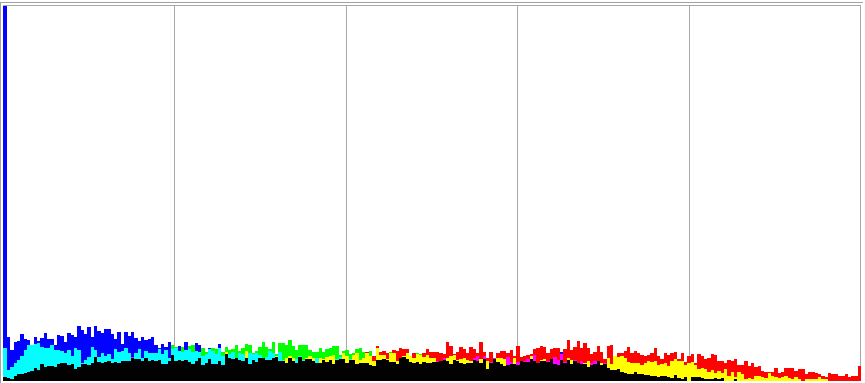
\includegraphics[width=.4\textwidth]{figures/gtOutHisto.png}}
		\caption{Samme besked, forskellige metoder}
	\end{figure}
\end{frame}

\begin{frame}[fragile]{Testabilitet}
	Mange private metoder
	\begin{itemize}
		\item Fleksibilitet %mht. implementering
		\item Lav testabilitet
	\end{itemize}
	\begin{itemize}
		\only<2->{\item{\lstinline{PrivateObject} \& \lstinline{PrivateType}}}
		\only<2->{\item{\ldots Eller udelukkende public?}}
	\end{itemize}
\end{frame}

\section{Konklusion}
\begin{frame}{Konklusion}
	Fokus på
	\begin{itemize}
		% Fcuk dis shiet
		\item{\sout{Sociale medier} $\rightarrow$ Diskrethed}
		\item JPEG encoder
		\item Studieordning:
		\begin{itemize}
			\only<2->{\item<pro@1->[\checkmark] Problemafgrænsning}
			\only<3->{\item<pro@1->[\checkmark] Model}
			\only<4->{\item<pro@1->[\checkmark] Større program}
			\only<5->{\item<pro@1->[\checkmark] Test}
			\only<6->{\item<pro@1->[\checkmark] Analysere problemorienteret projektarbejde}
		\end{itemize}
	\end{itemize}
\end{frame}
